\section{Benutzeradministration}\label{sect:useradministration}

Durch einen Klick auf das in Abbildung \ref{img:iconUsers} dargestellte Symbol, das sich in der Navigationsleiste oberhalb jeder Seite findet, gelangt man in das \ATFROGSnosp-Modul zur Benutzeradministration. In diesem Modul lassen sich bestehende Benutzer einsehen und l�schen. Au�erdem kann das Passwort eines Benutzers auf das in der Konfigurationsdatei \texttt{web.xml} definierte Standardpasswort (siehe Abschnitt \ref{sect:install:konfigurationsdateien}) zur�ckgesetzt werden.

\begin{figure}[htp]
   \centering
   
\includegraphics[scale=1]{graphics/userlogo.png}
   \caption{Icon des \ATFROGSnosp-Moduls zur Benutzeradministration}
   \label{img:iconUsers}
\end{figure}

\subsection{Auswahl eines Benutzers}\label{sect:useradministration:auswahlbenutzer}
�ber das mit {\small{\texttt{Benutzername:}}} beschriftete Eingabefeld ist eine Suche nach Benutzern aus der Menge der \OPENXCHANGE-Benutzer m�glich. Hierzu muss ein Suchmuster in das Eingabefeld eingetragen werden. Das Sternchen (\texttt{*}) kann als Platzhalter f�r beliebig lange Zeichenfolgen genutzt werden und darf innerhalb des Suchmusters beliebig oft auftreten.\footnote{In Abbildung \ref{img:user_overview} erscheint als Ergebnis der Suchanfrage \texttt{*ueller*} der Name Hans Mueller -- in der Annahme, dass dessen Benutzername \textit{Mueller} ist. Die Anfragen \texttt{Mueller} und \texttt{*ueller} w�rden zu demselben Ergebnis f�hren. W�rde ein Benutzer mit dem Benutzernamen \textit{Muellermeyer} existieren, so w�rde auch dieser in der Ergebnisliste der Anfrage \texttt{*ueller*} erscheinen, in der Ergebnisliste der beiden anderen Anfragen hingegen nicht. Zu beachten ist, dass das Sternchen (\texttt{*}) auch als Platzhalter f�r eine leere Zeichenfolge stehen kann.} Die Suche wird durch einen Klick auf 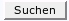
\includegraphics[scale=0.6]{graphics/button_search2.png} gestartet. Das Suchergebnis wird anschlie�end in der Liste unterhalb des Eingabefeldes dargestellt (siehe Abbildung \ref{img:user_overview}).\\

\begin{figure}[htp]
   \centering
   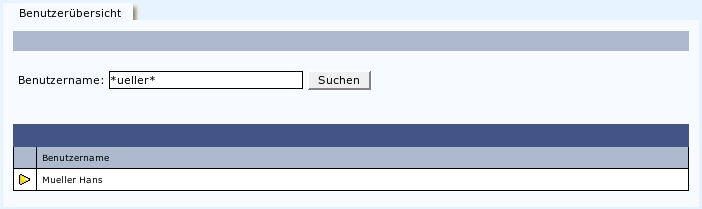
\includegraphics[width=\textwidth]{graphics/user_overview}
   \caption{Suche nach einem Benutzer}
   \label{img:user_overview}
\end{figure}

\NOTE{Durchsucht werden die Benutzernamen (UIDs) der Benutzer. Andere Felder wie Vorname oder Nachname werden nicht durchsucht!}\\[1cm]

\pagebreak

Nach einer erfolgreichen Suche ist es m�glich, sich die Details zu einem Benutzer anzusehen. Dazu muss auf den Benutzernamen in der Liste unterhalb des Eingabefeldes geklickt werden. Anschlie�end erscheint die Detailansicht zu dem Benutzer (siehe Abbildung \ref{img:user_details}).
\begin{figure}[htp]
   \centering
   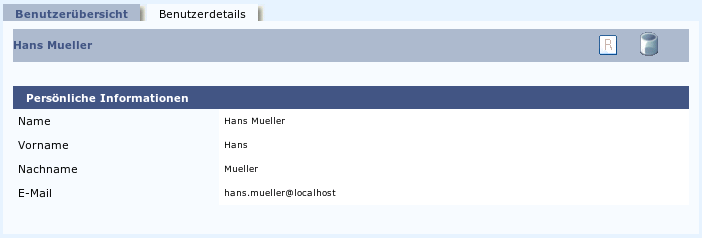
\includegraphics[width=\textwidth]{graphics/user_details}
   \caption{Detailansicht eines Benutzers}
   \label{img:user_details}
\end{figure}

\subsection{Zur�cksetzen des Passworts}\label{sect:useradministration:resetuserpwd}
Vorausgesetzt das Skript \textit{resetuserpwd} ist installiert (siehe Abschnitt \ref{sect:install:editweb.xml}), so kann das Passwort f�r einen Benutzer zur�ckgesetzt werden. Daf�r muss zun�chst einmal der entsprechende Benutzer gesucht und ausgew�hlt werden (siehe Abschnitt \ref{sect:useradministration:auswahlbenutzer}).\\

In der Detailansicht kann nun durch einen Klick auf 
\includegraphics[scale=0.6]{graphics/icon_reset.png} das Passwort des zuvor ausgew�hlten Benutzers zur�ckgesetzt werden. Nachdem der Wunsch best�tigt wurde, ist die Operation durchgef�hrt.

\subsection{L�schen eines Benutzers}
Um einen \OPENXCHANGE-Benutzer zu l�schen, muss dieser zun�chst einmal gesucht und ausgew�hlt werden (siehe Abschnitt \ref{sect:useradministration:auswahlbenutzer}).\\

In der Detailansicht kann der Benutzer durch einen Klick auf \ICON{graphics/icon_trash.png} gel�scht werden. Nachdem der Wunsch best�tigt wurde, ist der Benutzer endg�ltig gel�scht.\